\documentclass[12pt]{exam}
\newcommand{\hwnumber}{11 \& 12}
\newcommand{\hwname}{The C0VM}
\newcommand{\duedate}{\formatdate{25}{11}{\YEAR} % day-month-year
  and\\\phantom{\textbf{Due: }}\formatdate{5}{12}{\YEAR} by \progDueTime}

\usepackage{../misc/latex/edition}  % Course semester
\usepackage{../misc/latex/c0}       % Listings style for c0
\usepackage{amsmath}
\usepackage{enumerate}
\usepackage[normalem]{ulem}
\usepackage{verbatim}
\usepackage[left=1in, right=1in, top=1in, bottom=1in]{geometry}
\usepackage{graphicx}
\usepackage{hyperref}
\usepackage{tikz}     \usetikzlibrary{shapes}
\usepackage{fancybox}
\usepackage[all]{xy}
\usepackage{wrapfig}
\usepackage{fancyvrb}
\usepackage{datetime}
\usepackage{etoolbox}
\usepackage{calc}
\usepackage[nomessages]{fp}
\usepackage{import}  % Like input and include, but respects subdirectories

\newcommand{\defaultQuestionLocation}{questions}
\newcommand{\inputQuestion}[2][\defaultQuestionLocation/]{%
  \subimport{#1}{#2}
}
% Subdirectories of \defaultQuestionLocation containing code and pictures
\newcommand{\code}{code}
\newcommand{\img}{img}


%%% ic: frontmatter macros
\newcommand{\specialInstructions}{}
\newcommand{\HWNUMBER}
{\ifdefempty{\hwnumber}{__}{%
  \ifnumless{\hwnumber}{10}{0\hwnumber}{\hwnumber}}}
\newcommand{\hwtype}{Written Homework}

%%% ic: 'exam' tweaks
\renewcommand{\half}{.5} % Half points

\newcommand{\Question}[2][]
 {\ifstrempty{#1}
    {\question{\bf #2}}
    {\question[#1]{\bf #2}}
  \immediate\write\rubricfile{}%
  \immediate\write\rubricfile{Question \thequestiontitle:}%
  \immediate\write\rubricfile{==========}
 }

%%% ic: Support for editable PDF
% counter name (some viewers misbehave if always the same)
\newcounter{editable}
\newcommand{\nextField}{\addtocounter{editable}{1}q\arabic{editable}}
\newcommand{\NextField}
 {\makebox[0pt][r]{\scalebox{0.1}{\color{White}\nextField}}}

% Color of edit area
\newcommand{\editAreaColor}{red}
% Single line answer:   \editableLine[extra parameters (optional)]{line width}
\newcommand{\editableLine}[2][]
{\textcolor{\editAreaColor}{%
 \underline{\hspace*{-0.25em}%
 \raisebox{-0.5ex}{%
 \TextField[width=#2, borderwidth=0, #1]{\NextField}}}}%
}
% Single line answer for code:  \editableLine[extra parameters (optional)]{line width}
\newcommand{\editableCodeLine}[2][]
{\textcolor{\editAreaColor}{%
 \underline{%
 \TextField[width=#2, height=1.5ex, borderwidth=0, #1]{\NextField}}}}
% Multiline answer:  \editableLine[extra parameters (optional)]{box height}
\newcommand{\editableBox}[2][]
{\leavevmode\hspace*{-0.1em}%
\TextField[height=#2, width=\linewidth,
           multiline=true, borderwidth=0.1, bordercolor=\editAreaColor,
           #1]{\NextField}}

%%%%% Same answer format as exams
\renewcommand{\rmdefault}{ppl}
\renewcommand{\sfdefault}{phv}
\newcommand{\answerColor}{Blue}

\ifprintanswers
\newcommand{\answer}[2]{\makebox[#1][c]{\color{\answerColor}#2}}
\else
\newcommand{\answer}[2]{\makebox[#1][c]{}\makebox[0pt]{\phantom{|}}}
\fi
\newcommand{\uanswer}[2]{\underline{\answer{#1}{#2}}}


%%% Write rubric snippet.  Usage:
% \RUBRIC
% any multi-line text (including \, #, %, whatever)
% ENDRUBRIC
%% (ENDRUBRIC should be on a line by itself)
\makeatletter
\def\RUBRIC
 {%
  \begingroup
  \let\do\@makeother\dospecials
  \endlinechar=`\^^J
  \@tofile%
 }
\def\ENDRUBRIC{ENDRUBRIC}
\def\@tofile#1^^J{%
  \def\@test{#1}%
  \ifx\@test\ENDRUBRIC
    \immediate\write\rubricfile{}  % End with an empty line
    \expandafter\@firstoftwo
  \else
    \expandafter\@secondoftwo
  \fi
  {\endgroup}%
  {\toks@{#1}%
   \begingroup\endlinechar=\m@ne
   \everyeof{\noexpand}%
   \xdef\@temp{\scantokens\expandafter{\the\toks@}}%
   \endgroup
   \immediate\write\rubricfile{\@temp}%
   \@tofile}%
}
\makeatother

%% Displays tags for an exercise in 'answer' mode
\newcommand{\TAGS}[1]
{\ifprintanswers%
  \rule{0em}{0ex}%
  \marginpar{\footnotesize%
    \fcolorbox{black}{Gray!25}{%
      \parbox[t]{2cm}{\raggedright\textbf{TAGS:}\\#1}}}%
  \ignorespaces%
 \fi}%


%% Page layout
\pagestyle{headandfoot}

\headrule
\header{\textbf{\courseNumber{} \hwtype{} \hwnumber}}
       {}
       {\textbf{Page \thepage\ of \numpages}}
\footrule
\footer{}{}{\COPYRIGHT}

\renewcommand{\partlabel}{\textbf{\thequestion.\thepartno}}
%\renewcommand{\partlabel}{\textbf{Task \thepartno}}
\renewcommand{\subpartlabel}{\textbf{\thesubpart.}}
\renewcommand{\thepartno}{\arabic{partno}}
\renewcommand{\thesubpart}{\alph{subpart}}
\pointpoints{pt}{pts}
\pointformat{\raisebox{0ex}[\height][0pt]{\fcolorbox{black}{yellow}{\themarginpoints}}}
\bonuspointformat{\raisebox{0ex}[\height][0pt]{\fcolorbox{black}{red}{\themarginpoints}}}
\marginpointname{\points}
\pointsinmargin
%\boxedpoints

\setlength\answerlinelength{2in}
\setlength\answerskip{0.3in}

\newcommand{\mkWrittenTitle}[1]{#1}
\newcommand{\mkDueDate}[1]{#1}
\newcommand{\mkEvalSummary}[1]{#1}
\newcommand{\mkGradetable}[1]{#1}



% This fixes an issue with the exam package version 2.6 and after,
% where 'framed' has been renamed to 'examframed' to avoid a conflict.
\ifcsmacro{examframed}{%
\newenvironment{framed}
{\begin{examframed}}
{\end{examframed}}
}{}

\begin{document}
\hwTitle

\noindent
In this assignment you will implement a virtual machine for C0, the
C0VM\@.  It has been influenced by the Java Virtual Machine (JVM) and
the LLVM\@, a low-level virtual machine for compiler backends.  We
kept its definition much simpler than the JVM, following the design of
C0\@.  Bytecode verification, one of the cornerstones of the JVM
design, fell victim to this simplification; in this way the machine
bears a closer resemblance to the LLVM\@.  It is a fully functional
design and should be able to execute arbitrary C0 code.

The purpose of this assignment is to give you practice in writing C
programs in the kind of application where C is indeed often used in
practice.  C is appropriate here because a virtual machine has to
perform some low-level data and memory manipulation that is difficult
to make simultaneously efficient and safe in a higher-level language.
It should also help you gain a deeper understanding of how C0 (and, by
extension, C) programs are executed.

\bigskip
\noindent
The code handout for this assignment is at
\begin{center}
\whereisthetgz{c0vm-handout.tgz}
\end{center}
The file \lstinline'README.txt' in the code handout goes over the
contents of the handout and explains how to hand the assignment in.
There is a TWENTY (20) PENALTY-FREE HANDIN LIMIT for the \colorbox{orange}{checkpoint},
and a TWENTY (20) PENALTY-FREE HANDIN LIMIT for the full assignment.
Every additional handin for each will incur a small (5\%) penalty (even if
using a late day).
\emph{The checkpoint is for Tasks 1 and 2 only.  This is far, far less
  than half the assignment.}

After the checkpoint, you can no longer earn points for Tasks 1 and 2,
although the full autograder will continue to run tests against them.
It will also run tests for Tasks 3 and 4, \emph{but not for Task 5
  until after the handin deadline has passed.}  This means that you
must do all your own testing for Task 5 and in order to earn full
points you must convince yourself that you fully understand it and
have tested it for correct behavior and for memory leaks where
appropriate (you will see later in the writeup that certain memory
leaks are unavoidable).


\subsection*{About this writeup}

The C0VM is defined in stages, and we have test programs which
exercise only part of the specification.  We strongly recommend that
you construct your implementation following these stages and debug and
test each stage (on your own \emph{and} with the autograder) before
moving on to the next.  Each part has its own challenges, but each
part should be relatively small and self-contained.

This document describes the structure of the C0VM first and then the
instruction set (bytecodes) for the C0VM. After this, the document
will describe the tasks you need to perform, step by step. Read this
document very carefully as you prepare to do your work.

\section{The Structure of the C0VM}

Compiled code to be executed by the C0 virtual machine is represented
in a byte code format, typically stored in a file ending in extension
\lstinline'.bc0' which we call the \emph{bytecode file}.  This file
contains numerical and string constants as well as byte code for the
functions defined in the C0 source.
% In this way, and in many other
% details, it is similar to the JVM00 we presented earlier in this
% course.
The precise form of this file is specified in
Appendix~\ref{sec:bc0-format} and in \lstinline'lib/c0vm.h'.

\subsection{The Type \texttt{c0\_value}}

C0 has so-called \emph{small types} \lstinline'int', \lstinline'bool',
\lstinline'char', \lstinline'string', \lstinline't[]', and
\lstinline't*'.  Values of these types can be passed to or from
functions and held in variables. In the C0VM, we will represent each
of these types in one of two ways: the \emph{primitive types} are
represented as 32-bit signed integers (which we will abbreviate as
``\lstinline'w32''') and the \emph{reference types} are represented as
void pointers (which we will abbreviate as ``\lstinline'*''').

\begin{center}
\begin{tabular}{ccc}
C0 type & C0VM type & C type \\ % & ``op type'' (rec'd)\\
\hline
\texttt{int} & \texttt{w32} & \lstinline'int32_t' \\ % & \texttt{unsigned int} \\
\texttt{bool} & \texttt{w32} & \lstinline'int32_t' \\ % & \\
\texttt{char} & \texttt{w32} & \lstinline'int32_t' \\ % & \texttt{char} \\
\texttt{t[]} & \texttt{*} & \texttt{void*} \\ % & \texttt{c0\_array*} \\
\texttt{t*} & \texttt{*} & \texttt{void*} \\ % & \texttt{byte*}
\end{tabular}
\end{center}

In \lstinline'lib/c0vm.h', we create a special type \lstinline'c0_value' of C0
values. A \lstinline'c0_value' can store \emph{both} values of primitive
type (which we write as \lstinline'x', \lstinline'i', or \lstinline'n') and values of
reference or pointer type (which we write as \lstinline'a'). We can turn
primitive types into C0 values with the function \lstinline'int2val', and
we can turn C0 values which we know to be primitive types back into
integers with \lstinline'val2int'. Similarly, \lstinline'ptr2val(x)' and
\lstinline'val2ptr(x)' move between reference types (represented by
\lstinline'void*') and C0 values. We always have
\lstinline'val2int(int2val(x)) == x' for any integer $x$ and
\lstinline'val2ptr(ptr2val(a)) == a' for any pointer $a$. There's a
function \lstinline'val_equal(v1,v2)' which checks whether the two C0
values \lstinline'v1' and \lstinline'v2' are equal.

%% A correct implementation running well-formed bytecode should never
%% running \lstinline'val2int' on a value created with \lstinline'ptr2val'.

%%  cannot
%% not happen in well-formed bytecode.


%% We think of the small types as constituting two classes: the
%% \emph{primitive types} \lstinline'int', \lstinline'bool', and \lstinline'char' and
%% the \emph{reference types} \lstinline'string', \lstinline't[]' and \lstinline't*'.
%% All primitive types are conflated in the C0VM and denoted by
%% \lstinline'w32', indicating a 32 bit word.  Values of primitive types
%% are denoted by $x$, $i$, or $n$.  We also conflate all reference types
%% and write \lstinline'*'.  Values of reference type are denoted by $a$ for
%% \emph{address}.  An address uses either 32 bits or 64 bits.  On
%% the Linux machines you use, it will be 64 bits.

%% In addition C0 has \emph{large types} \lstinline'struct s' which cannot be
%% passed directly, but must be stored in memory.  When the C0VM executes
%% a program, it stores values of large type on \emph{its} heap and
%% refers to them by their address.  Calculations of how to access struct
%% fields are performed statically by the compiler, which computes proper
%% offsets for each access.  In addition, arrays (referenced by values of type
%% \lstinline't[]'), memory cells (referenced by values of type \lstinline't*') and
%% strings (referenced by values of type \lstinline'string') are stored on the
%% heap.

\subsection{Runtime Data}

The C0VM defines several types of data that are used during the
execution of a program. You'll need to consider the first three of
these (the operand stack, bytecode, and the program counter) to get
started with Task 1.

The \lstinline'execute' function you are extending in this assignment is
passed a struct \lstinline'bc0_file' containing all the information from
the bytecode. As you read this section, you should refer to both
Appendix~\ref{sec:bc0-format} and \lstinline'lib/c0vm.h' where this struct
is described.

\subsubsection{The Operand Stack (S)}

The C0VM is a \emph{stack machine}, similar in design to Clac and the
JVM\@.  This means arithmetic operations and other instructions pop
their operands from an operand stack and push their result back onto
the operand stack.
%This is in contrast with \emph{register machines}
%where instructions such as arithmetic operations act on a finite set
%of registers.

The C0VM is defined in terms of operand stack \lstinline'S', a stack of C0
values. Because these values are such an important part of the VM, we
define stacks that only contain C0 values in
\lstinline'lib/c0v_stack.h'. We recommend writing some helper functions
like \lstinline'push_int(S, i)' and \lstinline'pop_ptr(S)' early on so that you
won't have to repetitively write \lstinline'c0v_push(S, int2val(i))' and
\lstinline'val2ptr(c0v_pop(S))' over and over.

\subsubsection{Bytecode (P)}

In Clac, the program instructions were strings, and they were stored
in a queue of strings. In the C0VM, instructions for the current C0
function are stored in an array of (unsigned) bytes %
(\lstinline'ubyte *P'). %
Each function in a compiled C0 program is represented by a struct
\lstinline'function_info' that is stored in the array
\lstinline'bc0->function_pool'. The \lstinline'main()' function that
you want to run first is always stored as the first struct in this
array, at index 0. When you start your VM, you should initialize
\lstinline'P' to be the bytecode \lstinline'code' stored in that
struct.

You don't ever need to allocate any memory to store bytecode. Just
refer to the bytecode given to the \lstinline'execute' function.

\subsubsection{The Program Counter (pc)}

The program counter \lstinline'pc' holds the address of the program
instruction currently being executed.  It always starts at 0 when you
begin executing a function. Unless a non-local transfer of control
occurs (goto, conditional branch, function call or return), the
program counter is incremented by the number of bytes in the current
instruction before the next instruction is fetched and interpreted.

\subsubsection{Local variables (V)}

Locals should be stored in a \lstinline'c0_value' array. Every struct
\lstinline'function_info' has a field \lstinline'num_vars' which
specifies how big this array needs to be in order to store all the
locals of that function. The four components \lstinline'S',
\lstinline'P', \lstinline'pc', and \lstinline'V' are everything that
we need to know in order to represent the current state of any
function.

\subsubsection{The Call Stack}

The C0VM has a call stack consisting of \emph{frames}, each one
containing local variables, a local operand stack, and a return
address.  The call stack grows when a function is called and shrinks
when a function returns, deallocating the frame during the return.

Every frame consists of the four components that represent the current
state of some function call that got interrupted in order to call
another function.  It contains the operand stack \lstinline'S' for
computing expression values, a pointer \lstinline'P' to the function's byte
code, a return address \lstinline'pc', which is the address of the next
instruction in the interrupted function, and an array of locals
\lstinline'V'. At any point during the execution there is a \emph{current
  frame} as well as a \emph{calling frame}. The latter becomes the
current frame when a function returns to its caller.

\subsubsection{Constant Pools}

Numerical constants requiring more than 8 bits and all string
constants occurring in the program will be allocated in constant
pools, called the \emph{integer pool} and the \emph{string pool}.  They never
change during program execution.


\subsubsection{Function Pools}

Functions, either C0 functions defined in a source file or library
functions, are kept in pools called the \emph{function pool} and the
\emph{native pool}, respectively.  Functions in the function pool are
stored with their bytecode instructions, while functions in the native
pool store an index into a table of C function pointers that the C0VM
implementation can dereference and invoke.


\subsubsection{The Heap}

At runtime, the C0 heap contains C0 strings, C0 arrays (\lstinline't[]')
and C0 cells (\lstinline't*').  C0 arrays have to store size information so
that dynamic array bounds checks can be performed.  You will
use the C heap to implement the C0 heap: that is, you will
allocate strings, arrays, and cells directly using calls to
\lstinline'xmalloc' and \lstinline'xcalloc' as defined earlier in this course.

Since C0 is designed as a garbage-collected language, you will not be
able to free space allocated on behalf of C0 unless you are willing
to implement (or use) a garbage collector.  We do not view this as a
memory leak of the C0VM implementation.  On the other hand, temporary
data structures required for the C0VM's own operation should be properly
freed.

This means that when you are testing your own code using \lstinline'valgrind',
you must be aware of which \texttt{bc0} files should be free of
\lstinline'valgrind' memory leak reports and which should produce reports of
memory leaks. The autograder will not penalize \lstinline'valgrind' reports of
memory leaks for tests that allocate space on the C0 heap.

Note that the autograder will also not penalize for memory leaks for tests that
are supposed to end in a runtime error.

%\subsection{Frames}


%% Since values of small type may occupy 4 bytes or 8 bytes, the data
%% structures implementing frames, including the array of local variables
%% and the operand stack, all work in terms of the type \lstinline'c0_value',
%% which is a type that can contain either an 8 byte pointer or a 4 byte
%% integer. We define an inline function \lstinline'int2val(x)' to cast an
%% integer $x$ to a \lstinline'c0_value', and a converse \lstinline'val2int(x)' to
%% cast a C0 value back to an integer. Similarly, \lstinline'ptr2val(x)' and
%% \lstinline'val2ptr(x)' move between pointer types (represented by
%% \lstinline'void*') and C0 values. We always have
%% \lstinline'val2int(int2val(x)) == x' for any integer $x$ and
%% \lstinline'val2ptr(ptr2val(p)) == p' for any pointer $p$. Incorrectly
%% running \lstinline'val2int' on a value created with \lstinline'ptr2val' cannot
%% not happen in well-formed bytecode. %% By keeping around some extra informa

%% Every C0 value is represented in the VM
%% by either a pointer or an integer (see Section~\ref{sec:prolif}), so we
%% only need these four functions.

%% allocate 8 bytes for each data value, whether
%% of primitive type or reference type.  From the C perspective, things
%% are simplest if these are of type \lstinline'void*', but to clarify intent,
%% we create a type alias \lstinline'c0_value', defined to be \lstinline'void*',
%% for arbitrary C0 values.  This strategy requires us to be able to cast
%% ints to pointers and vice versa without loss of information. The C99
%% standard leaves this behavior implementation-defined, but the Andrew
%% version of \lstinline'gcc' implements such casts.  We define an inline
%% function \lstinline'VAL(x)' to cast an integer $x$ to a \lstinline'c0_value',
%% and a converse \lstinline'INT(p)' to cast a pointer $p$ to a 32-bit signed
%% integer (an \lstinline'int32_t').  For the latter to work, $p$ must have
%% been created with a \lstinline'VAL(x)' cast, otherwise the result is
%% unpredictable except for \lstinline'NULL' (which returns 0).  So we always
%% have \lstinline'INT(VAL(x)) == x' for any integer $x$.

%% The \lstinline'main' function we have provided (see the file
%% \lstinline'c0vm_main.c') performs some simple tests to verify that casts
%% between \lstinline'void*' and \lstinline'int' do not lose information.  If any
%% of these tests fail, C0VM will abort with an appropriate error
%% message.


\subsection{Runtime Errors}

In order to fully capture the behavior of C0 programs, you must
correctly issue errors for things like dereferencing \lstinline"NULL",
indexing an array outside of its bounds, and dividing by zero.
Check the C0 Language Reference for details on what kinds of errors
you must handle, and then use the following provided functions
(defined in \lstinline'c0vm_abort.h' and \lstinline'c0vm_abort.c') to issue
appropriate error messages:
%\begin{quote}
\begin{lstlisting}[numbers=none]
void c0_user_error(char *err);         // for calls to error() from C0
void c0_assertion_failure(char *err);  // for failed assertions from C0
void c0_memory_error(char *err);       // for memory-related errors
void c0_arith_error(char *err);        // for arithmetic-related errors
\end{lstlisting}
%\end{quote}
For unexpected situations that arise while executing bytecode, situations
which could indicate a bug in your VM, you may use the standard C library
functions \lstinline"abort" or \lstinline[language=C]"assert" to abort your
program. See Section~\ref{sect:assertions} for more details on this
distinction.

\section{Instruction Set}

We group the instructions by type, in order of increasing complexity
from the implementation point of view.  We recommend implementing them
in order and aborting with an appropriate message when an unimplemented
instruction is encountered. Each task in this assignment corresponds
to one or more sections,
and tasks are summarized in Section~\ref{sec:testing}.


\subsection{Stack Manipulation (Task 1)}
\label{sec:stack}

There are three instructions for direct stack manipulation without
regard to types.

\begin{lstlisting}[language=opsem]
0x59 dup           S, v -> S, v, v
0x57 pop           S, v -> S
0x5F swap          S, v1, v2 -> S, v2, v1
\end{lstlisting}

\subsection{Arithmetic Instructions (Task 1)}
\label{sec:arith}

Arithmetic operations in C0 are defined using modular arithmetic based
on a two's complement signed representation.  This does not match your
implementation language (C) very well, where the result of
\emph{signed} arithmetic overflow is undefined. There are two
solutions to this problem: first, because \emph{unsigned} arithmetic
overflow is defined to be modular arithmetic, you could cast
\lstinline'int32_t' values to \lstinline'uint32_t', perform unsigned
arithmetic, then cast back. This should not be required in your
implementations, however: we will compile your code with the
\lstinline'-fwrapv' command-line argument that forces \lstinline'gcc'
to treat integer arithmetic to be defined as signed two's complement
arithmetic.  (Remember, however, that this is not part of the C
standard.)

Casting signed integers to unsigned integers and/or using the
\lstinline'-fwrapv' command-line argument does not do everything that is
needed to ensure C0 compliance, but it goes a long way.  We recommend
a careful reading of the arithmetic operations in the
\href{http://c0.typesafety.net/doc/c0-reference.pdf}{C0 Reference}, as
well as the notes on casting integers in C.

For this implementation strategy to be correct, it is important to
verify that our C environment does indeed use a two's complement
representation and that the C type of \lstinline'int' has 32 bits.
The provided \lstinline'main' function (see the file
\lstinline'c0vm_main.c') performs these checks before starting the
abstract machine and aborts the execution if necessary.

In the instruction table below (and for subsequent tables), we use
\lstinline'w32' for the type of primitive values and \lstinline'*' for
the type of reference values.  Each line has an opcode in hex
notation, followed by the operation mnemonic, followed by the effect
of the operation, first on the stack, then any other effect.
\begin{lstlisting}[language=opsem]
0x60 iadd         S, x:w32, y:w32 -> S, x+y:w32
0x7E iand         S, x:w32, y:w32 -> S, x&y:w32
0x6C idiv         S, x:w32, y:w32 -> S, x/y:w32
0x68 imul         S, x:w32, y:w32 -> S, x*y:w32
0x80 ior          S, x:w32, y:w32 -> S, x|y:w32
0x70 irem         S, x:w32, y:w32 -> S, x%y:w32
0x78 ishl         S, x:w32, y:w32 -> S, x<<y:w32
0x7A ishr         S, x:w32, y:w32 -> S, x>>y:w32
0x64 isub         S, x:w32, y:w32 -> S, x-y:w32
0x82 ixor         S, x:w32, y:w32 -> S, x^y:w32
\end{lstlisting}
Safety violations in \lstinline[language=opsem]'idiv',
\lstinline[language=opsem]'irem', \lstinline[language=opsem]'ishr',
and \lstinline[language=opsem]'ishl' can cause run-time errors (use
the provided function \lstinline"c0_arith_error" to generate a
message).  Please refer to the C0 language specification for important
details.

We have omitted negation \lstinline'-x', which the compiler can simulate
with \lstinline'0-x', and bitwise negation \lstinline'~x', which the compiler
can simulate with \lstinline'x^(-1)'.

\subsection{Constants (Tasks 1 and 2)}
\label{sec:constants}

We can push constants onto the operand stack.  There are three
different forms: (1) a constant \lstinline'null' which is directly coded
into the instruction, (2) a small \emph{signed} (byte-sized) constant
\lstinline'<b>' which is an instruction operand and must be sign-extended
to 32 bits, and (3) a constant stored in the constant pool.  For the
latter, we distinguish constants of primitive type from those of
reference type because they are stored in different pools.

The two constant loading instructions \lstinline[language=opsem]'ildc'
and \lstinline[language=opsem]'aldc' take two unsigned bytes as
operands, which must be combined into an unsigned integer index for
the appropriate constant pool.  The integer pool stores the constants
directly, and the index given to \lstinline[language=opsem]'ildc' is
an index into the integer pool.  The string pool is one large array of
character strings, each terminated by \lstinline"'\0'".  The index
given to \lstinline[language=opsem]'aldc' indicates the position of
the first character; its address is therefore of type
\lstinline'char*' in C and understood by C as a string.

\begin{lstlisting}[language=opsem]
0x01 aconst_null   S -> S, null:*
0x10 bipush <b>    S -> S, x:w32     (x = (w32)b, sign extended)
0x13 ildc <c1,c2>  S -> S, x:w32     (x = int_pool[(c1<<8)|c2])
0x14 aldc <c1,c2>  S -> S, a:*       (a = &string_pool[(c1<<8)|c2])
\end{lstlisting}
You will not be able to test \lstinline[language=opsem]'aldc' in any
interesting way until you implement \lstinline[language=opsem]'athrow'
or \lstinline[language=opsem]'assert' (see below).


\subsection{Local Variables (Task 2)}
\label{sec:local}

We can move data generically between local variables and the stack,
because all primitive types can fit into pointers or integers and so
be stored as a \lstinline'c0_value'. %% size of a reference
%% type (\lstinline'c0_value', which is defined as \lstinline'void*',
%% is 8 bytes on 64-bit systems).
The instruction operand \lstinline[language=opsem]'<i>' is one byte
following the opcode \lstinline[language=opsem]'0x15' or
\lstinline[language=opsem]'0x36' in the instruction stream.  Because
this is the only way to access a local variable, each function can
have at most 256 local variables, which includes the function
arguments.

\begin{lstlisting}[language=opsem]
0x15 vload <i>      S -> S, v                     (v = V[i])
0x36 vstore <i>     S, v -> S                     (V[i] = v)
\end{lstlisting}

\subsection{Assertions and Errors (Task 2)}
\label{sec:asserts}

The instruction \lstinline[language=opsem]'athrow' implements the C0
built-in \lstinline'error(s)' which aborts execution with error
message \lstinline's'.  In the bytecode, this error message will be at
the top of the stack --- it will have been put there by
\lstinline'aldc' if it is a literal string.

The instruction \lstinline[language=opsem]'assert' implements all C0
contracts and assertions.  You will be able to use its full potential
only after you are done with Tasks 3 and 4.  For now, you can test it
with programs containing simple assertions like \lstinline'assert(true)' or
\lstinline'//@assert false;' (remember to compile the latter with the flag
\lstinline'-d').

\begin{lstlisting}[language=opsem]
0xBF athrow            S, a:* -> S          (c0_user_error(a))
0xCF assert            S, x:w32, a:* -> S   (c0_assertion_failure(a) if x == 0)
\end{lstlisting}


\subsection{Control Flow (Task 3)}
\label{sec:control}

Each instruction implicitly increments the program counter by the
number of bytes making up the instruction.  Control flow instructions
change this by jumping to another instruction under certain
conditions.  The addressing is relative to the address of the branch
instruction.  The offset is a \emph{signed} 16 bit integer that is
given as a two-byte operand to the instruction.  It must be signed so
we can branch backwards in the program.
% We distinguish pointer comparisons (only
% equality and inequality) from integer comparisons.
Note that \lstinline"if_cmpeq" and \lstinline"if_cmpne" can be used to
compare either integers or pointers for equality or inequality,
whereas the other comparisons only make sense on integers.  The
\lstinline[language=opsem]'nop' ``no-op'' instruction has no effect.

\begin{lstlisting}[language=opsem]
0x00 nop               S -> S

0x9F if_cmpeq <o1,o2>  S, v1, v2 -> S       (pc = pc+(o1<<8|o2) if v1 == v2)
0xA0 if_cmpne <o1,o2>  S, v1, v2 -> S       (pc = pc+(o1<<8|o2) if v1 != v2)
0xA1 if_icmplt <o1,o2> S, x:w32, y:w32 -> S (pc = pc+(o1<<8|o2) if x < y)
0xA2 if_icmpge <o1,o2> S, x:w32, y:w32 -> S (pc = pc+(o1<<8|o2) if x >= y)
0xA3 if_icmpgt <o1,o2> S, x:w32, y:w32 -> S (pc = pc+(o1<<8|o2) if x > y)
0xA4 if_icmple <o1,o2> S, x:w32, y:w32 -> S (pc = pc+(o1<<8|o2) if x <= y)

0xA7 goto <o1,o2>      S -> S               (pc = pc+(o1<<8|o2))
\end{lstlisting}

\subsection{Function Calls and Returns (Task 4)}
\label{sec:functions}

Function calls come in two forms: invoking a C0 function defined in
the same bytecode file and invoking a library function defined in C\@.
In either case, generic arguments \lstinline'v1' through
\lstinline'vn' are passed on the operand stack and consumed.  The C0VM
implementation must guarantee that the result \lstinline'v' is pushed
onto the stack when the function returns.  For functions returning
\lstinline'void', a dummy value is pushed onto the operand stack to
provide a uniform interface to functions.

Function information is stored in the function pool or native pool,
both of which are addressed by the instruction operand consisting of
two bytes, which must be reconstituted into an \emph{unsigned} 16 bit
quantity indexing into the appropriate pool.

\begin{lstlisting}[language=opsem]
0xB8 invokestatic <c1,c2> S, v1, v2, ..., vn -> S, v
                          (function_pool[c1<<8|c2] = g, g(v1,...,vn) = v)
0xB0 return   ., v -> .   (return v to caller)
\end{lstlisting}

When invoking a C0 function (instruction
\lstinline[language=opsem]'invokestatic') we have to preserve the
state of the calling function so that we can resume it later: a
pointer to its bytecode, its program counter \lstinline'pc' as a
return address, its current local variable array $V$ and its current
operand stack $S$.  This is the information in a \emph{frame} which is
pushed onto a global call stack.  Then we set the \lstinline'pc' to
the beginning of the code for the called function $g$, allocate a new
array of local variables, and initialize it with the function
arguments from the old operand stack.  We also create a new empty
operand stack for use in the called function.

When processing a \lstinline[language=opsem]'return' instruction we
restore the \lstinline'pc', the local variable array $V$ and the
operand stack $S$ from the last frame on the call stack.  We also need
to arrange that the return value is popped from the current operand
stack and pushed onto the operand stack of the frame we return to.
Some temporary data structures may need to be deallocated at this
point.

The \lstinline'main' function always has index $0$ in the function
pool and takes $0$ arguments.  After reading the file, setting up
appropriate data structures, etc, your C0VM implementation should
start executing byte code at the beginning of this function and at the
end print the final value.

%% In this assignment, you should use two instances of the abstract data type
%% of stacks, one holding frames (the call stack) the other holding
%% operands (the operand stack).%
%% \footnote{There are a number of other plausible implementation paths for the
%% two stacks.  One possibility is inspired by the system call stack for
%% languages such as C\@.  In this strategy there is one global array
%% storing return addresses, local variables, and (in the case of the
%% C0VM) also an area to use as the operand stack.  This implementation
%% would not use our abstract datatype of stacks, but implement the stack
%% as an array with a so-called stack pointer which is the current top of
%% the stack.  Of course, it is not really treated exactly like an
%% abstract stack, because the access to local variables violates the
%% pure stack discipline. Another possibility is to
%% have a single operand stack, shared throughout the execution,
%% rather than local ones for each frame.  This is possible because
%% the C0VM specification requires that when a function returns, its
%% operand stack must be empty.}
% Each of them is used just using pushes and pops, as the stack interface
% dictates.  Remember, your stacks or arrays will have to share data of
% different types, namely primitive types and reference types.

%% A reasonable mapping to C implementation types would be \lstinline'int32_t'
%% for primitive types and \lstinline'void*' for reference types, implementing
%% respectively the types \lstinline'w32' and \lstinline'*' in the description of
%% the instructions.  This allows you to store all C0VM values of small
%% type as type \lstinline'c0_value' and cast them to the appropriate type for
%% the operations you need to perform on them and to cast the result back
%% when finished.

\subsection{Native Function Calls (Task 4)}
\label{sec:native}

Native function calls have the same form as C0 function calls, but the
two-byte instruction argument indexes into the native pool, rather
than the function pool.
\begin{lstlisting}[language=opsem]
0xB7 invokenative <c1,c2> S, v1, v2, ..., vn -> S, v
\end{lstlisting}
The value \lstinline'native_pool[c1<<8|c2]' is a struct
\lstinline'native_info' (defined in \lstinline'lib/c0vm.h' and
described in Appendix~\ref{sec:bc0-format}), which contains two
fields: \lstinline'num_args', the number $n$ of arguments that should
be popped off the stack, and \lstinline'function_table_index', which
is an index $i$ into a separate runtime structure, the
\lstinline'native_function_table' (defined in
\lstinline'lib/c0vm_c0ffi.h'). From that table you can retrieve the
address of a function $g$, a pointer to a function taking an array of
\lstinline'c0_value' and returning a \lstinline'c0_value'.

% The type \lstinline'c0_value*' should be read as an array of
% pointers of type \lstinline'c0_value', which indicates generic data.
% It also returns a value of generic type.
In order to call this function you have to construct an array of
length~$n$ and store arguments \lstinline'v1' through \lstinline'vn'
at indices~$0$ through~$n-1$, and then invoke the function~$g$ on this
array.  The result has to be pushed back onto the operand stack.

Native function calls do not therefore involve explicitly managed
stack frames.  Of course, your abstract machine implementation is
using the system stack, so when you call the library function, the
library function also uses the system stack, rather than any stack
managed explicitly by your virtual machine.

The mapping between native library functions and their indices into
the native function table is
% important only if you wish to construct by hand bytecode files that
% invoke native functions, and it is
given as a series of \lstinline'NATIVE_*' macros in the file
\lstinline'c0vm_c0ffi.h'. (You will not need to use these definitions in
your C0VM implementation.)

\subsection{Memory Allocation, Load, and Store (Task 5)}
\label{sec:memory}

Besides function calls, the trickiest aspect of the C0VM
implementation is the management of the C0 runtime heap.
%There are
%two basic options.  One is to allocate on the C runtime heap (that is
%available to your C0VM implementation as it runs) one very large
%array and perform C0 allocations inside this array.  The type of
%references would then be \lstinline'int', values denoting array indices.
%Alternatively, y
Your implementation should satisfy each C0 allocation request separately
by allocating a sufficient amount of space on the C runtime heap,
using C pointers to implement C0VM references.
%The latter option is
%advantageous for the purpose of calling native functions because the C
%runtime heap is shared between the running C0VM implementation and the
%C0 bytecode program that it executes.
Your implementation
of allocation must take care to initialize all memory requested by C0
to all zeros.

\begin{lstlisting}[language=opsem]
0xBB new <s>       S -> S, a:*     (*a is now allocated, size <s>)
\end{lstlisting}

The \lstinline[language=opsem]'new <s>' instruction allocates $s$
bytes of memory ($s$ is an unsigned byte) and pushes the address of
the newly allocated memory (a pointer) onto the stack.  The data size
is computed statically by the C0 compiler.  For example, the C0
expression \lstinline'alloc(int)' would translate to
\lstinline[language=opsem]'new 4', while \lstinline'alloc(struct b)'
would translate to \lstinline[language=opsem]'new n', where $n$ is the
size of a \lstinline'struct b' in memory in bytes, which is always
known at compile time.

We read from and write to addresses in memory with the six
instructions: \lstinline[language=opsem]'imload' and
\lstinline[language=opsem]'imstore' for integers,
\lstinline[language=opsem]'amload' and
\lstinline[language=opsem]'amstore' for pointers, and
\lstinline[language=opsem]'cmload' and
\lstinline[language=opsem]'cmstore' for characters. For integers and
pointers, we treat the value on the stack as an integer or a pointer
and store that quantity directly. For characters, we have to be a bit
more careful, because characters (which may take on the values 0-127
in C0) are stored as integer values on the stack. When we read a
character out of memory we have to cast it to an integer, and when we
write we do the opposite, masking the given value of type
\lstinline'w32' to 7 bits.
\begin{lstlisting}[language=opsem]
0x2E imload    S, a:* -> S, x:w32   (x = *a, a != NULL, load 4 bytes)
0x4E imstore   S, a:*, x:w32 -> S   (*a = x, a != NULL, store 4 bytes)
0x2F amload    S, a:* -> S, b:*     (b = *a, a != NULL, load address)
0x4F amstore   S, a:*, b:* -> S     (*a = b, a != NULL, store address)
0x34 cmload    S, a:* -> S, x:w32   (x = (w32)(*a), a != NULL, load 1 byte)
0x55 cmstore   S, a:*, x:w32 -> S   (*a = x & 0x7f, a != NULL, store 1 byte)
\end{lstlisting}
For each operation, you must check that the
address~$a$ of a load or store instruction is non-NULL and raise a memory
error if~$a$ is NULL.

Most of the time, when we're reading and writing from memory in our C0
program, we're not using pointers directly to read (\lstinline'*p') or write
(\lstinline'*p=...'). Rather, we're reading from or writing to fields of
structs (\lstinline'T->data=...') or elements of arrays
(\lstinline'A[i]=...').  In the C0VM, these two steps are split into different
VM instructions for address arithmetic and loading from or storing to a
computed address. This computation then gives us the actual address of the
integer, pointer, or character stored within the array or struct, which we can
access with the six instructions above.

There are two kinds of offset computations: one for arrays, and one
for structs. When we access a struct's field, the compiler generates a
field offset $f$ (an unsigned one-byte quantity). The \lstinline[language=opsem]'aaddf'
instruction is used to add $f$ bytes to the pointer $a$ at the top of
the stack.  If the address~$a$ is NULL, you must raise a memory error
by calling the provided function \lstinline"c0_memory_error".

\begin{lstlisting}[language=opsem]
0x62 aaddf <f>      S, a:* -> S, (a+f):*  (a != NULL; f field offset)
\end{lstlisting}

In order to talk about array offsets, we need to talk about how C0
arrays are represented at runtime.  C0 arrays are represented as
pointers to a struct\footnote{defined in \texttt{lib/c0vm.h}.}
\lstinline'c0_array_header' that has three fields. The first,
\lstinline'count', is the number of elements in the array, and is
determined at runtime (this is \lstinline'n' in the
\lstinline'newarray' instruction below). The second,
\lstinline'elt_size', represents the number of bytes in a single
element; the compiler is able to determine this at compile time based
on the type (this is \lstinline's' in the
\lstinline[language=opsem]'newarray' instruction below).
\begin{center}
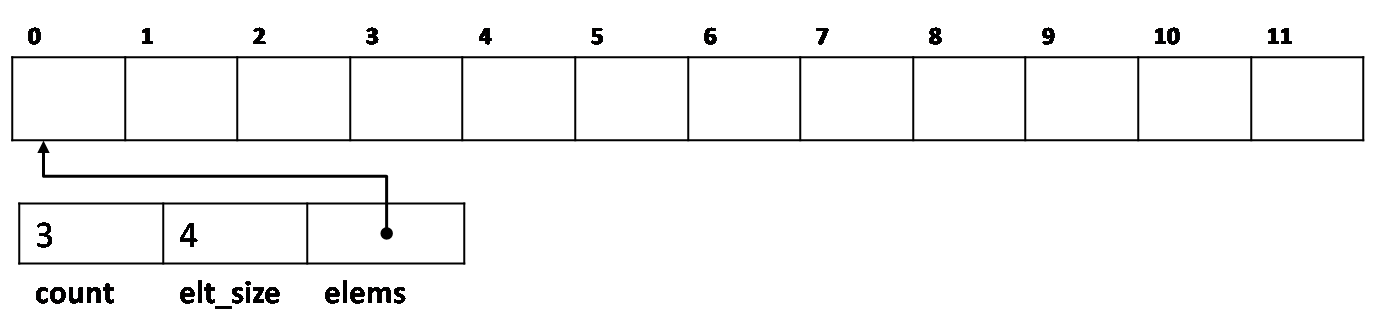
\includegraphics[width=0.8\textwidth]{img/c0_array_header.png}
\end{center}
The third field is \lstinline'elems', a void pointer to the beginning of the
memory allocated for the actual array, which contains \lstinline'n*s'
bytes. The length of an array, stored in the \lstinline'count' field, can
be retrieved with the \lstinline'arraylength' C0VM instruction.
Every C0 array
you encounter in the VM will be a pointer to one of these
structs.\footnote{It is possible for a C0 array to be
  {\tt NULL}; the VM should treat {\tt NULL} like an array with
  length 0.}

The picture above is an array of three objects with
\lstinline'elt_size' of 4, perhaps a C0 integer. The third integer
(array offset 2 in the C0 array) is stored in the bytes labeled
8-11. If we cast the void pointer in the \lstinline'elems' field to a
\lstinline'char' pointer named \lstinline'arr', then the offset we
should compute to access the third integer in the array is
\lstinline'&arr[2*4]' --- the address 8 bytes into the block of
allocated memory (array offset 2 $\times$ 4 bytes per array element;
recall that a char is defined to be one byte).

\begin{lstlisting}[language=opsem]
0xBC newarray <s>  S, n:w32 -> S, a:*     (a[0..n) now allocated)
0xBE arraylength   S, a:* -> S, n:w32     (n = \length(a))
0x63 aadds         S, a:*, i:w32 -> S, (a->elems+s*i):*
                                          (a != NULL, 0 <= i < \length(a))
\end{lstlisting}

The \lstinline[language=opsem]'newarray <s>' instruction allocates
memory for an array containing \lstinline'n' elements at size
\lstinline's'. The size is computed by the compiler, while the array
size is determined at runtime because it cannot in general be known at
compile time.  The \lstinline[language=opsem]'aadds' instruction
computes the address of an array element.  The operand~$a$ on the
stack must be the address of an array, and the operand~$i$ must be a
valid index for this array. The C0VM must issue an error message and
abort if~$i$ is not a valid index, which can be determined from the
stored array length; use the provided function
\lstinline"c0_memory_error" to issue this error.  We then use the
element size~$s$ stored with the array to compute the address of
the~$i$th element.  Note that one \lstinline[language=opsem]'aadds'
instruction is necessary for every array access, even if we access the
element at index~$0$.  This is in contrast to structs! When we are
accessing a field of a struct, we might be accessing the first field,
in which case the address of the field is the same as the address of
the struct.


\clearpage
\section{Programming Tasks and Coding Advice}

There are many complexities in implementing a virtual machine,
especially one that is rich enough so it can execute all of C0!
Fortunately, some of the complexities (such as parsing the bytecode
file) are taken care of by code we are providing, but others remain.
You will complete the code in \lstinline'c0vm.c'.

The following are suggested strategies to help you work effectively
throughout this project.

\subsection{Testing}\label{sec:testing}

We have provided a few test cases in \lstinline'tests/', but it is
more effective to write your own.  Write a small file, say
\lstinline'test.c0' and compile it with \lstinline'cc0 -b test.c0',
which will create a bytecode file \lstinline'test.bc0'.  Then run it
with \lstinline'./c0vmd test.bc0'.  Compare your answers with the ones
you get with \lstinline'cc0 -x mytest.c0':

\begin{lstlisting}[language={[coin]C}]
% cc0 -x tests/iadd.c0
-2
% cc0 -b tests/iadd.c0
% ./c0vmd tests/iadd.bc0
Opcode 10 -- Stack size: 0 -- PC: 0
Opcode 10 -- Stack size: 1 -- PC: 2
Opcode 60 -- Stack size: 2 -- PC: 4
Opcode b0 -- Stack size: 1 -- PC: 5
Returning -2 from execute()
-2
\end{lstlisting}


\subsection{Incremental Implementation}\label{sec:tasks}

Implement a subset of the instruction set and test your C0VM
implementation on code that only uses the subset.  Generate some test
cases using \lstinline'cc0 -b' from simple C0 sources, or use some of the
supplied examples that use limited instructions.  You should recognize
instructions that are valid but not in your subset and give a
``\emph{not yet implemented}'' message and returning rather than
aborting in the same way as for other errors.  Test one stage
thoroughly before moving on.  After extending the machine, first make
sure the old, simple examples still run correctly, a process called
\emph{regression testing}.  The stages follow our discussion of
the instruction set:

\begin{task}[15]
\TAGS{c0vm, stack}
[See Sections~\ref{sec:stack} and~\ref{sec:arith}]\\
Initialize the variables
\lstinline'S',
\lstinline'P' and
\lstinline'pc'
correctly in the \lstinline'execute' function in the
\lstinline'c0vm.c' file.

Add code to handle arithmetic instructions, plus
\lstinline[language=opsem]'bipush', \lstinline[language=opsem]'swap',
and \lstinline[language=opsem]'return'.  (The return instruction is
mostly implemented, but needs to be checked for memory leaks.) C0
programs with only a \lstinline'main' function returning an expression
made of small constants can be used to test these capabilities, e.g.,
\enlargethispage{1ex}
\begin{lstlisting}
int main() {
  return 15 * ((1<<10) - 24) + 122;
}
\end{lstlisting}
\end{task}


\begin{task}[10]
  \TAGS{c0vm, c-numbers, c-memory}
  [See Sections~\ref{sec:constants}, \ref{sec:local} and~\ref{sec:asserts}]\\
  Add code to deal with local variables, constants and assertions;
  you'll need to initialize the variable \lstinline'V' to something
  better than \lstinline'NULL'.  C0 source files containing
  straight-line code using variables and large constants can be used
  to test these capabilities, e.g.,
\begin{lstlisting}
int main() {
  int x = 15122;
  assert(true);
  int y = x * x;
  return y;
}
\end{lstlisting}
\end{task}

\noindent%
\colorbox{orange}{\makebox[\linewidth]{\rule[-1ex]{0em}{4ex}\textbf{CHECKPOINT}}}


\begin{task}[7]
\TAGS{c0vm, c-numbers}
[See Section~\ref{sec:control}]\\
 Add code to handle \lstinline[language=opsem]'goto' and conditionals
(e.g., \lstinline[language=opsem]'if_icmpge').
  Now you should be able to execute loops, as in
\begin{lstlisting}
int main () {
  int i; int sum = 0;
  for (i = 15; i <= 122; i++)
    sum += i;
  return sum;
}
\end{lstlisting}
\end{task}

\begin{task}[10]
\TAGS{c0vm, c-numbers, c-memory, stack}
  [See Sections~\ref{sec:functions} and~\ref{sec:native}]\\
  Add function calls (\lstinline[language=opsem]'invokestatic',
  \lstinline[language=opsem]'invokenative'); you'll probably want to
  initialize the variable \lstinline'callStack' to something better
  than \lstinline'NULL' and use \lstinline'callStack' to manage the
  call stack in some form. You will also need to revisit
  \lstinline[language=opsem]'return' (see \lstinline'PROG_HINTS.txt'
  in the code handout).  You may want to focus on ordinary C0 function
  calls (\lstinline[language=opsem]'invokestatic',
  \lstinline[language=opsem]'return') before moving on to native
  function calls (\lstinline[language=opsem]'invokenative').

Now your \lstinline'main' function can call auxiliary functions,
  such as the ubiquitous recursive factorial function, and
  library functions that print output:
\begin{lstlisting}
int factorial(int n) {
  return n == 0 ? 1 : n * factorial(n-1);
}
int main () {
  printint(factorial(15));
  println(" is the factorial of 15");
  return 0;
}
\end{lstlisting}
\end{task}

\begin{task}[8]
\TAGS{c0vm, c-numbers, c-memory}
[See Section~\ref{sec:memory}]\\
 Add the C0 heap, where arrays and structs are
  allocated.
  % This is likely to be the biggest step.
  After this, you should be
  able to run arbitrary C0 code, including your own C0 assignments.
\end{task}


\subsection{Assertions}
\label{sect:assertions}

Ideally, we would establish invariants of the bytecode that we read
from a file to make sure no runtime memory or type error occurs.  In
the JVM this is referred to as \emph{bytecode verification}.
Unfortunately, the current bytecode format does not provide enough
information to do this.  Even if it did, it would be a major
project in itself.  So you have to fall back on dynamic checks.
These checks come in two categories:
\begin{enumerate}
\item%
  The usual checks on the runtime structure of your own code,
  verifying that pointers are not \lstinline'NULL', etc.
\item%
  Checks that the C0 bytecode you have read in behaves properly.
\end{enumerate}
Some of the checks in the second category are mandated:
\begin{enumerate}[(a)]
\item%
  The C0 program must not dereference the C0 \lstinline'NULL' pointer
  or perform pointer arithmetic on it.
\item%
  The C0 program must not access memory outside the bounds of a C0 array.
\item%
  The C0 program must not perform illegal integer division (division
  by 0, or the min int divided by -1).
\item%
  The C0 program must not shift left or right by a number $< 0$ or
  $\geq 32$.
\end{enumerate}
If you encounter these runtime errors, you should produce error
messages using the provided functions
\smallskip
\begin{itemize}
\item%
  \lstinline"void c0_memory_error(char *err)" --- for memory-related errors
\item%
  \lstinline"void c0_arith_error(char *err)" --- for division or shift-related
  errors
\end{itemize}
\smallskip%
By calling these functions, which are declared in
\lstinline'c0vm_abort.h', you make it clear that this is a runtime
error in the bytecode you are executing and not a bug in your machine.

The first category of checks should in principle be redundant.  For
example, the \lstinline'cc0' compiler should never produce a bytecode
file that jumps to an invalid address.
% , that is, the current \lstinline'pc' plus the
% offset of a jump is not a valid address in the current code array.
Nevertheless, bytecode written by hand or a bug in the \lstinline'cc0'
compiler or your VM could lead to such issues.  Since C does not
guarantee detection of such incorrect jumps or accesses, your code
should do that using appropriate \lstinline'assert' statements, or
\lstinline'ASSERT', \lstinline'REQUIRES', and \lstinline'ENSURES'.
Then, if the bytecode itself or your virtual machine implementation
has a bug, it will be discovered as soon as an unexpected incorrect
behavior occurs.  The macro annotations are recommended so that there
is no undue overhead for correct code when your machine has been
debugged.

%% \subsection{The Proliferation of Types}
%% \label{sec:prolif}

%% One common issue in writing virtual machines and similar (almost)
%% self-referential code is the proliferation of different types at
%% different levels, sometimes with the same name.  It will be important
%% for you to understand the various level of types involved, whether
%% they are signed or unsigned, and what they refer to.  In addition you
%% will have to cast between types for various operations.

%% The following table might help.  The C type is only recommended, not
%% required.
%% \[\begin{tabular}{ccc}
%% C0 type & C0VM type & C type (recommended) \\ % & ``op type'' (rec'd)\\
%% \hline
%% \texttt{int} & \texttt{w32} & \lstinline'int32_t' \\ % & \texttt{unsigned int} \\
%% \texttt{bool} & \texttt{w32} & \lstinline'int32_t' \\ % & \\
%% \texttt{char} & \texttt{w32} & \lstinline'int32_t' \\ % & \texttt{char} \\
%% \texttt{t[]} & \texttt{*} & \texttt{void*} \\ % & \texttt{struct c0\_array*} \\
%% \texttt{t*} & \texttt{*} & \texttt{void*} \\ % & \texttt{byte*} \\
%% \texttt{struct s} & (none) & (none) \\ % & \\
%% function & function pool index & \texttt{struct function\_info} \\ % & \\
%% library fn & native pool index & \texttt{struct native\_info} \\ % & \texttt{void*(*native\_fn)(void**)}
%% \end{tabular}\]
%% Sometimes you will have to cast the C type that represent the C0VM types
%% to a form where they are appropriate for the operation to be performed
%% on them.  An example of this are the arithmetic operations, which
%% are reliably performed on unsigned ints so we have to cast to and
%% from these types.


\subsection{Manage Your Time Well}

Remember that this homework is worth \textbf{50 points}, and the last
three tasks are \emph{much} more difficult than the first two. You
should plan on working on this for an hour or two every day, so you
can ask for help early on if you need it. \textbf{Don't wait until the
  last few days!}  Post general questions on \qatool{} (e.g., questions
about the C0VM specification, wording of tasks, requirements for
handin, etc).

\clearpage
\appendix
\section{Bytecode File Format}
\label{sec:bc0-format}

The bytecode file, usually with extension \lstinline'.bc0', is
produced by the \lstinline'cc0' compiler when invoked with the
\lstinline'-b' or \lstinline'--bytecode' flag. In order to allow you
to easily read bytecode, and also write your own bytecode, the binary
file is coded in hexadecimal form, where two-digit bytes are separated
by whitespace.  In addition, the file may contain comments starting
with `\lstinline"#"' and extending to the end of the line.

We describe the format as pseudo-structs, where we use the types
described below.  For multi-byte types, each byte is given separately
by two hexadecimal digits, with the most significant byte first.

\medskip
\begin{tabular}{l@{ \ --- \ }l}
   \lstinline'u4' & 4 byte unsigned integer
\\ \lstinline'u2' & 2 byte unsigned integer
\\ \lstinline'u1' & 1 byte unsigned integer
\\ \lstinline'i4' & 4 byte signed (two's complement) integer
\\ \lstinline'fi' & struct \lstinline'function_info', defined below
\\ \lstinline'ni' & struct \lstinline'native_info', defined below
\end{tabular}

\medskip
\noindent
The size of some arrays is variable, depending on earlier fields.
These are only arrays conceptually, of course.  In the file,
all the information is just stored as sequences of bytes separated
by whitespace.

\begin{lstlisting}[language=C, morecomment={[l]\#}]
struct bc0_file {
  u4 magic;                          # magic number, always 0xc0c0ffee
  u2 version+arch;                   # version number and architecture
  u2 int_count;                      # number of integer constants
  i4 int_pool[int_count];            # integer constants
  u2 string_count;                   # number of characters in string pool
  u1 string_pool[string_count];      # adjacent '\0'-terminated strings
  u2 function_count;                 # number of functions
  fi function_pool[function_count];  # function info
  u2 native_count;                   # number of native (library) functions
  ni native_pool[native_count];      # native function info
};
\end{lstlisting}

\begin{lstlisting}[language=C, morecomment={[l]\#}]
struct function_info {
  u2 num_args;                       # number of arguments, V[0..num_args)
  u2 num_vars;                       # number of variables, V[0..num_vars)
  u2 code_length;                    # number of bytes of bytecode
  u1 code[code_length];              # bytecode
};
\end{lstlisting}

\begin{lstlisting}[language=C, morecomment={[l]\#}]
struct native_info {
  u2 num_args;                      # number of arguments, V[0..num_args)
  u2 function_table_index;          # index into table of library functions
};
\end{lstlisting}

We are providing code that reads bytecode files and marshals the
information into similar internal C structures.

\section{C0VM Instruction Reference}

What follows is a reference for the C0VM bytecode, which is also given
as part of the handout (\lstinline'c0vm-ref.txt'). Every line that
describes an operation has the following format:

\begin{lstlisting}[language=opsem]
0xYZ omne         S -> S' (other effect)
\end{lstlisting}

\noindent
where \lstinline'0xYZ' is the opcode in hex, \lstinline'omne' is the
operation mnemonic, and the remaining text describes the effect of the
operation. The description includes the effect on the stack
(e.g. transform stack \lstinline'S' into stack \lstinline"S'") and any
other effects (e.g. modify the program counter).

\bigskip

\lstinputlisting[language=opsem]{../src/c0vm-ref.txt}

\end{document}
